\documentclass[12pt]{report}
    \title{\textbf{CAP4630 Intro to Artificial Intelligence \\ Knowledge-based
Intelligent System \\ Project 3 - Report}}
    \author{Tobias Dault, Eyob Tekle, William L. Thomson Jr.}
    \date{April 1st, 2022}

    \addtolength{\textheight}{3cm}
	\usepackage{enumitem}
    \usepackage{hyperref}
    \usepackage{float}
    \usepackage{graphicx}
    \usepackage{subcaption}
    \usepackage[tmargin=1in,lmargin=1in,rmargin=1in]{geometry}
	\usepackage{titlesec}
	
    \DeclareCaptionFormat{custom}
    {%
        \textbf{\footnotesize #1#2}\textit{\footnotesize #3}
    }
    \captionsetup{format=custom}

    \graphicspath{ {./assets/} }

	\hypersetup{ colorlinks=true, linkcolor=blue, filecolor=purple, urlcolor=cyan }

    \newlength\tindent
    \setlength{\tindent}{\parindent}
    \setlength{\parindent}{0pt}
    \renewcommand{\indent}{\hspace*{\tindent}}

    \setlist[description]{noitemsep, topsep=0pt, itemsep=.5em}
    \setlist[enumerate]{noitemsep, topsep=0pt, itemsep=.5em}
    \setlist[itemize]{noitemsep, topsep=0pt, itemsep=.5em}

    \titleformat{\chapter}
	{\Large\bfseries}
	{\thechapter.}{0.5em}{}

	\titleformat{\section}
	{\large\bfseries}
	{\thesection.}{0.5em}{}

	\titleformat{\subsection}
	{\normalsize\bfseries}
	{\thesubsection.}{0.5em}{}

    \titlespacing\chapter{0pt}{12pt plus 0pt minus 4pt}{0pt plus 0pt minus 4pt}
    \titlespacing\section{0pt}{12pt plus 4pt minus 8pt}{0pt plus 2pt minus 8pt}
    \titlespacing\subsection{0pt}{12pt plus 4pt minus 2pt}{0pt plus 2pt minus 2pt}

\begin{document}

\maketitle
\tableofcontents
\thispagestyle{empty}

\chapter{Overview}
\section{About}
This program is a knowledge-based intelligent system that collects user preferences and reasons about them. The program collects names of attributes, values of attributes ($A$), hard constraints represented as propositional formulas in conjunctive normal form (CNF) ($H$), and preferences languages of penalty logic, possibilistic logic, and qualitative choice logic with preference formulas ($T$) also in conjunctive normal form (CNF) from user input or files with the purpose of performing the following four reasoning tasks: \\

\begin{description}[style=multiline,leftmargin=12em]
  \item [Existence of Feasible Objects] Whether there are feasible objects w.r.t $H$,
that is, whether there are models of $H$ that are truth assignments making $H$ true.
  \item [Exemplification] Generate two random feasible objects, and show the preference between the two (strict preference or equivalence) w.r.t $T$
  \item [Optimization] Find an optimal object w.r.t $T$
  \item [Omni-Optimization] Find all optimal objects w.r.t $T$
\end{description}

\section{Design}
The program is written in Python and leverages the Tkinter python binding to TK GUI toolkit, used for the GUI of the program. The belowlying logic is mostly performed with the use of clasp, an answer set solver for normal and disjunctive logic programs. The program wraps the clasp binary and uses it to perform tasks such as existence of feasible objects and for penalty and possibilistic preference logics. Qualitative choice logic is performed internally in the programs code without the use of clasp.


\chapter{Input}
The program relies upon user input for all functionality, either from direct user input via text input form fields and the add buttons, or by file upload of properly formatted files using the open file buttons, or a combination of user input and file upload. Without such input, the program will not function, and it will prompt the user for missing attributes, hard constraints, and/or preferences before performing any of the intended functions. All input and related actions are performed under the input tab.

\section{Binary Attributes}
The first required input are the binary attributes. The program requires at least one or more binary attributes to function. Binary attributes can be entered in one by one, or in bulk via a file upload, which is recommended. Additional attributes can be entered directly in addition to those loaded from a file.

\newpage
\subsection{Input Binary Attributes from a File}
The following steps are based on using the open file method of inputting attributes.\\

\begin{description}[leftmargin=4em]
\item [Step 1:] Click the \textbf{"Open File"} button below the Binary Attributes table
\begin{figure}[H]
\begin{center}
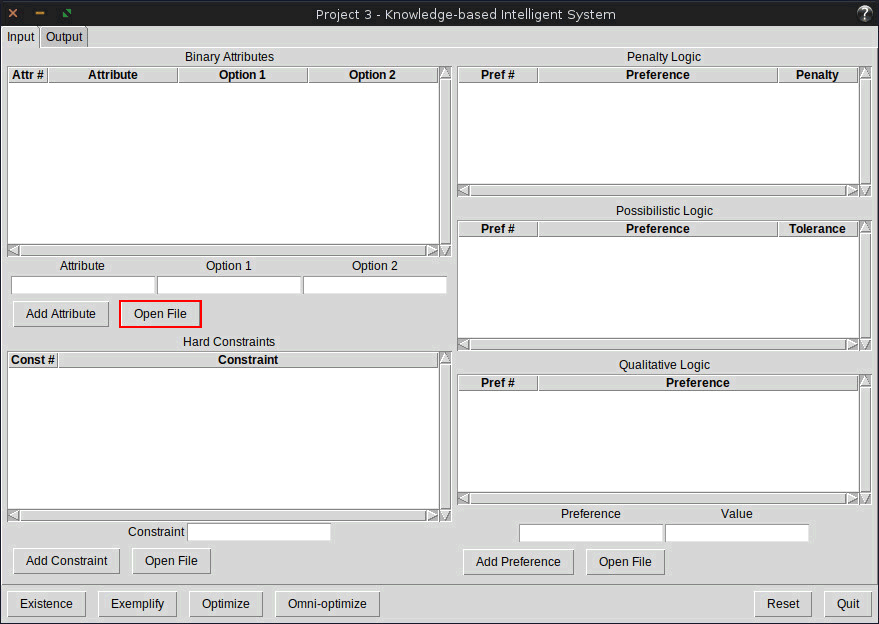
\includegraphics[scale=0.275,trim=1cm 1cm 1cm 1cm]{input_attributes}
\caption{Screenshot of selecting attributes from a file}
\end{center}
\end{figure}
\vspace{-2.5em}
\item [Step 2:] Select the desired file (attributes$\_$test.txt for this example) and click \textbf{"Open"}.
\begin{figure}[H]
\begin{center}
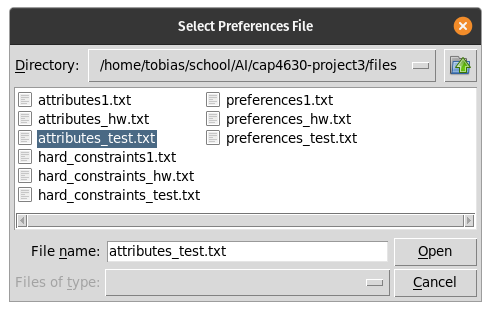
\includegraphics[scale=0.3,trim=1cm 1cm 1cm 1cm]{select_attributes}
\caption{Screenshot of selecting a attributes text file}
\end{center}
\end{figure}
\vspace{-2.5em}
\item [Result:] The contents of the file will be displayed in the \textbf{Binary Attributes table}
\begin{figure}[H]
\begin{center}
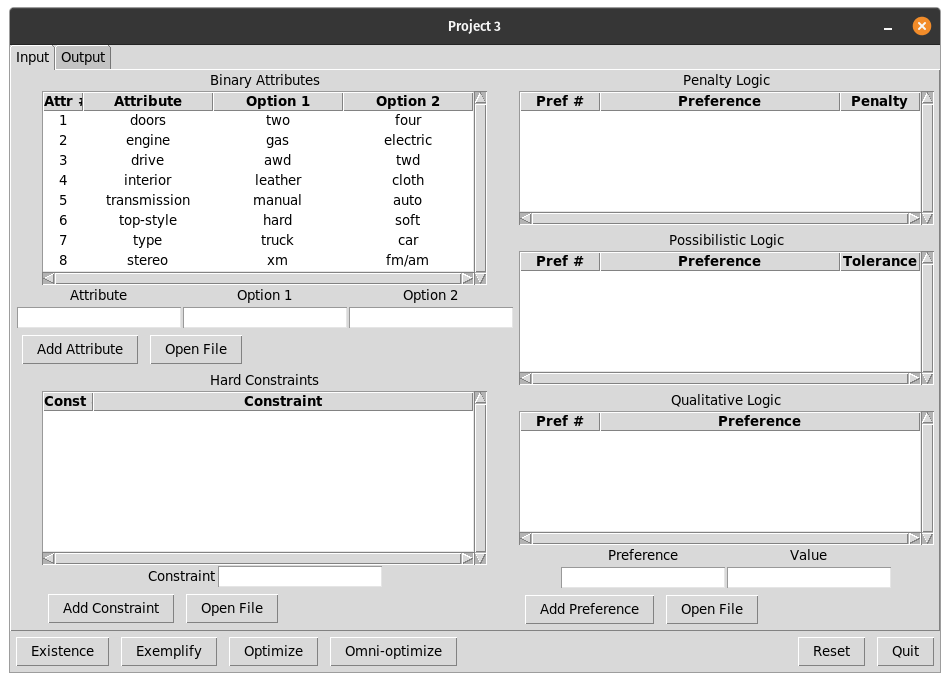
\includegraphics[scale=0.275,trim=1cm 1cm 1cm 1cm]{attributes_imported}
\caption{Screenshot of attributes loaded from file}
\end{center}
\end{figure}
\vspace{-2.5em}
\end{description}

\section{Hard Constraints}
The second required input are the hard constraints. The program requires at least one or more hard constraints to function. Hard constraints can be entered in one by one, or in bulk via a file upload, which is recommended. Additional hard constraints can be entered directly in addition to those loaded from a file.

\newpage
\subsection{Input Hard Constraints from a File}
The following steps are based on using the open file method of inputting hard constraints.\\

\begin{description}[leftmargin=4em]
\item [Step 1:] Click the \textbf{"Open File"} button below the Hard Constraints table
\begin{figure}[H]
\begin{center}
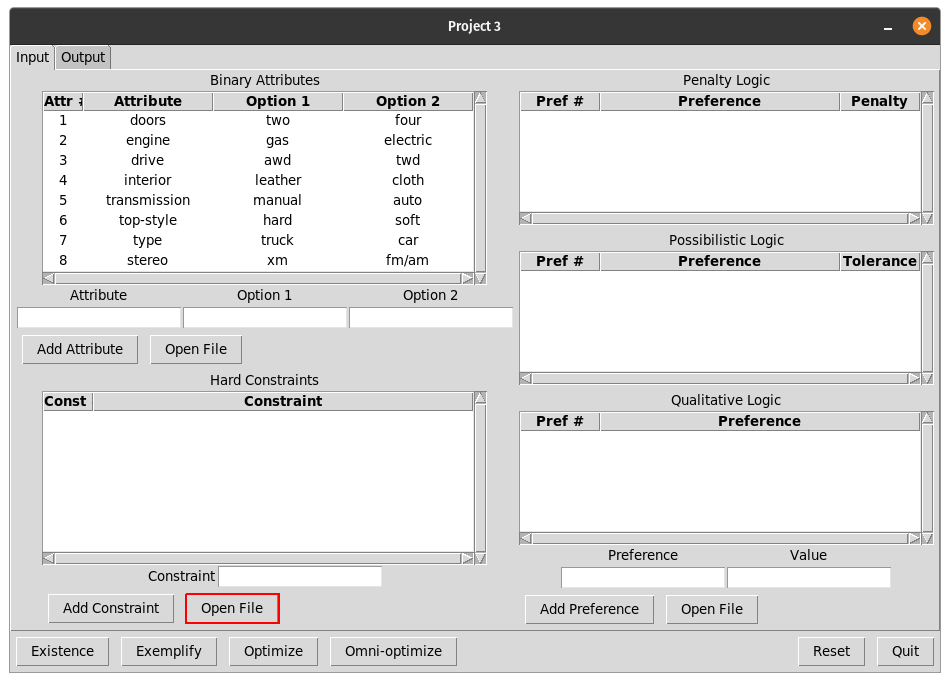
\includegraphics[scale=0.275,trim=1cm 1cm 1cm 1cm]{input_constraints}
\caption{Screenshot of selecting hard constraints from a file}
\end{center}
\end{figure}
\vspace{-2.5em}
\item [Step 2:] Select the desired file (hard$\_$constraints$\_$test.txt for this example) and \textbf{"Open"}.
\begin{figure}[H]
\begin{center}
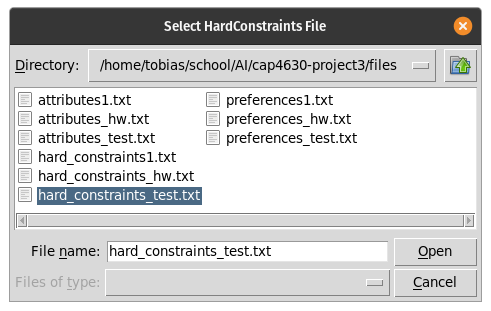
\includegraphics[scale=0.3,trim=1cm 1cm 1cm 1cm]{select_constraints}
\caption{Screenshot of selecting a hard constraints text file}
\end{center}
\end{figure}
\vspace{-2.5em}
\item [Result:] The contents of the file will be displayed in the the \textbf{Hard Constraints table}
\begin{figure}[H]
\begin{center}
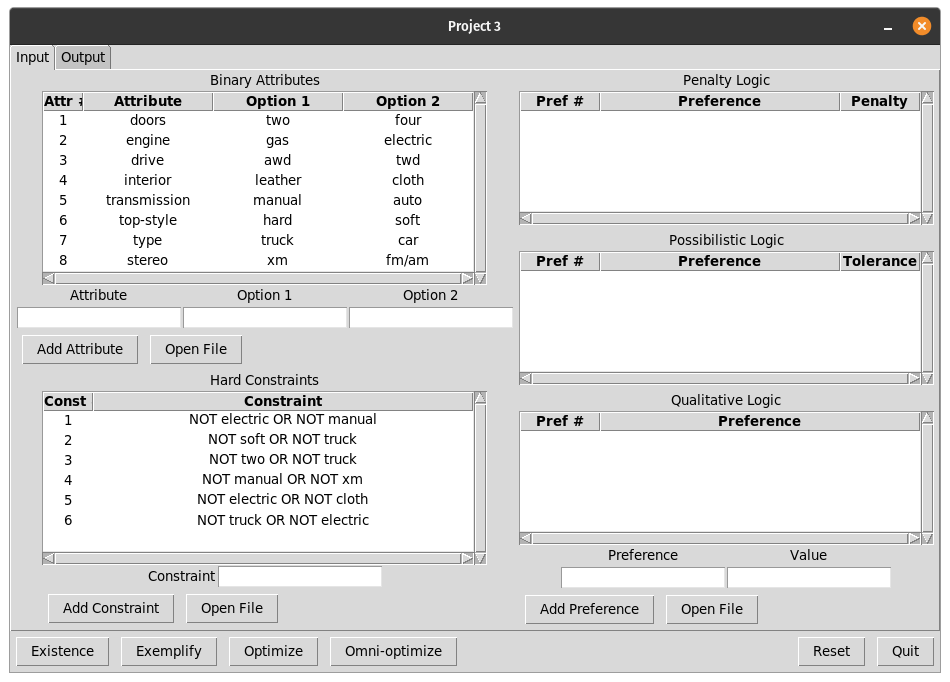
\includegraphics[scale=0.275,trim=1cm 1cm 1cm 1cm]{constraints_imported}
\caption{Screenshot of hard constraints loaded from file}
\end{center}
\end{figure}
\vspace{-2.5em}
\end{description}

\section{Preference Logics}
The third and final required input are the preference logics: penalty logic, possibilistic logic, and qualitative choice logic. The program requires at least one or more preference logics for each of the three types to function. Preference logics can be entered in one by one, or in bulk via a file upload, which is recommended. Additional preference logics can be entered directly in addition to those loaded from a file. The type of logic will be automatically determined based on the value, if one exists, which it does not for qualitative choice logic.

\newpage
\subsection{Input Preference Logics from a File}
The following steps are based on using the open file method of inputting preference logics.\\

\begin{description}[leftmargin=4em]
\item [Step 1:] Click the \textbf{"Open File"} button below the three Preference Logics tables
\begin{figure}[H]
\begin{center}
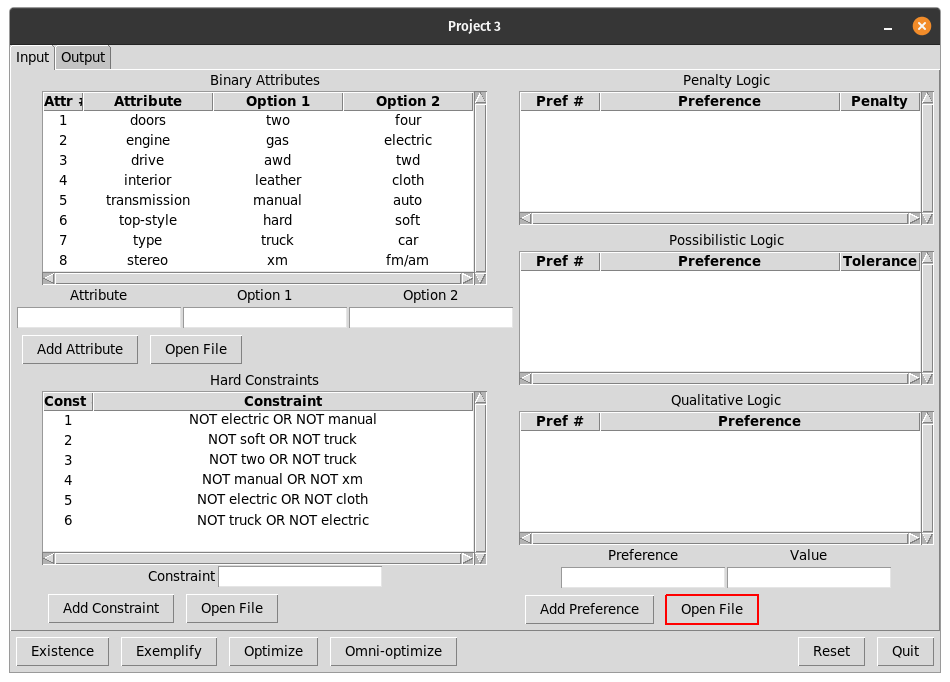
\includegraphics[scale=0.275,trim=1cm 1cm 1cm 1cm]{input_preferences}
\caption{Screenshot of selecting preference logics from a file}
\end{center}
\end{figure}
\vspace{-2.5em}
\item [Step 2:] Select the desired file (preferences$\_$test.txt for this example) and click \textbf{"Open"}.
\begin{figure}[H]
\begin{center}
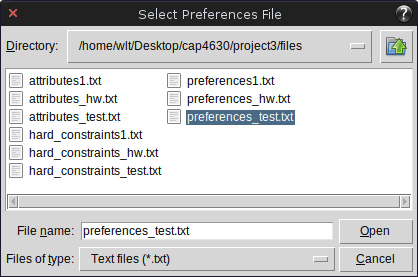
\includegraphics[scale=0.3,trim=1cm 1cm 1cm 1cm]{select_preferences}
\caption{Screenshot of selecting a preference logics text file}
\end{center}
\end{figure}
\vspace{-2.5em}
\item [Result:] The contents of the file will be displayed in the \textbf{three Preference Logics tables}
\begin{figure}[H]
\begin{center}
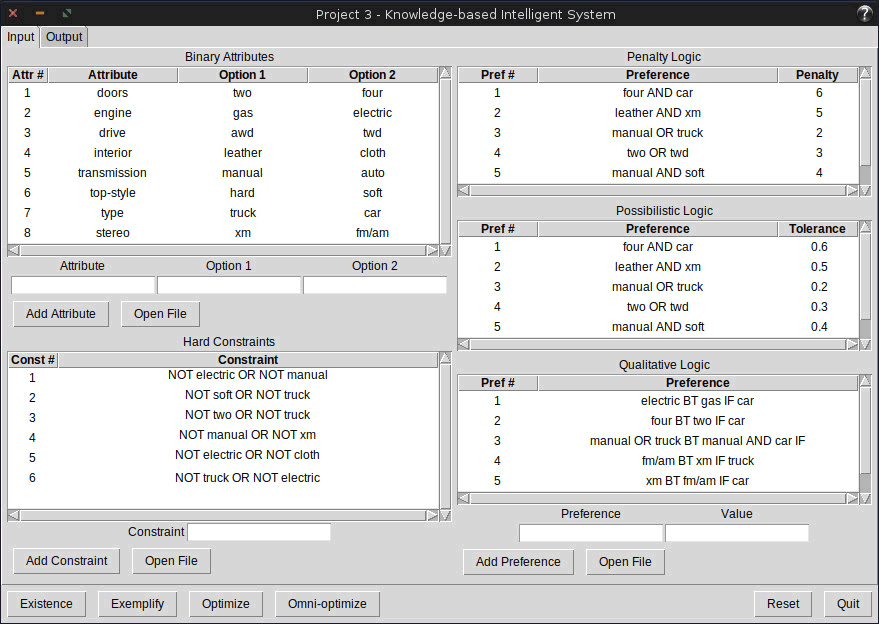
\includegraphics[scale=0.275,trim=1cm 1cm 1cm 1cm]{preferences_imported}
\caption{Screenshot of preference logics loaded from file}
\end{center}
\end{figure}
\vspace{-2.5em}
\end{description}


\chapter{Output}
\section{Existence of Feasible Objects}
The following steps demonstrate the existence of feasible objects functionality of the program.\\

\begin{description}[leftmargin=4em]
\item [Step 1:] Click the \textbf{"Existence"} button
\begin{figure}[H]
\begin{center}
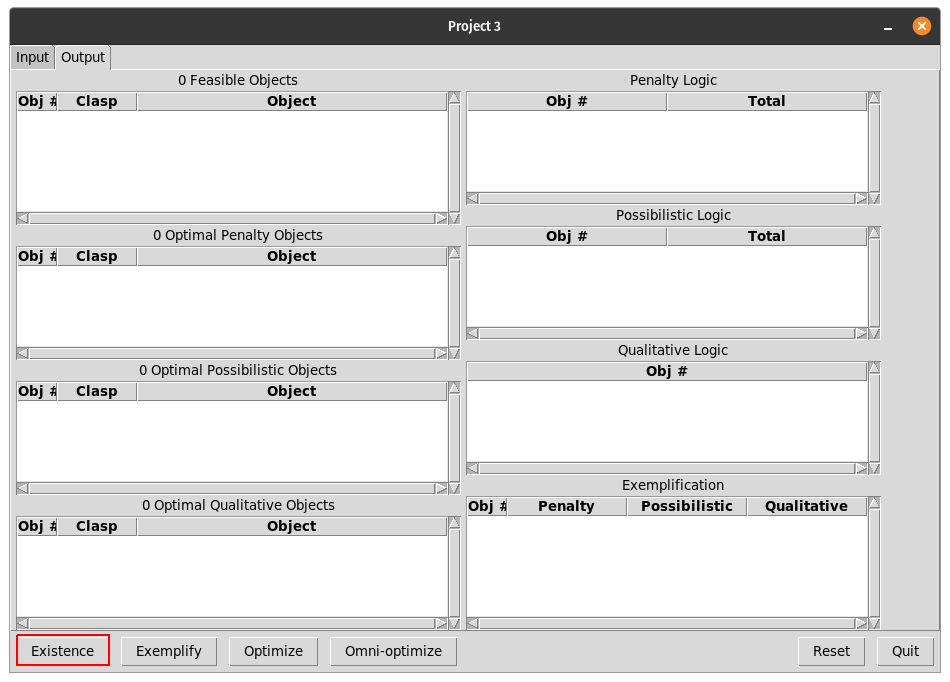
\includegraphics[scale=0.3,trim=1cm 1cm 1cm 1cm]{existence}
\caption{Screenshot of clicking the existence button}
\end{center}
\end{figure}
\vspace{-2.5em}
\item [Result:] All feasible objects will be displayed in the \textbf{feasible objects table} on the output tab, along with the total number of feasible objects. The output tab will be auto-focused on button click if on input tab when the button is clicked.
\begin{figure}[H]
\begin{center}
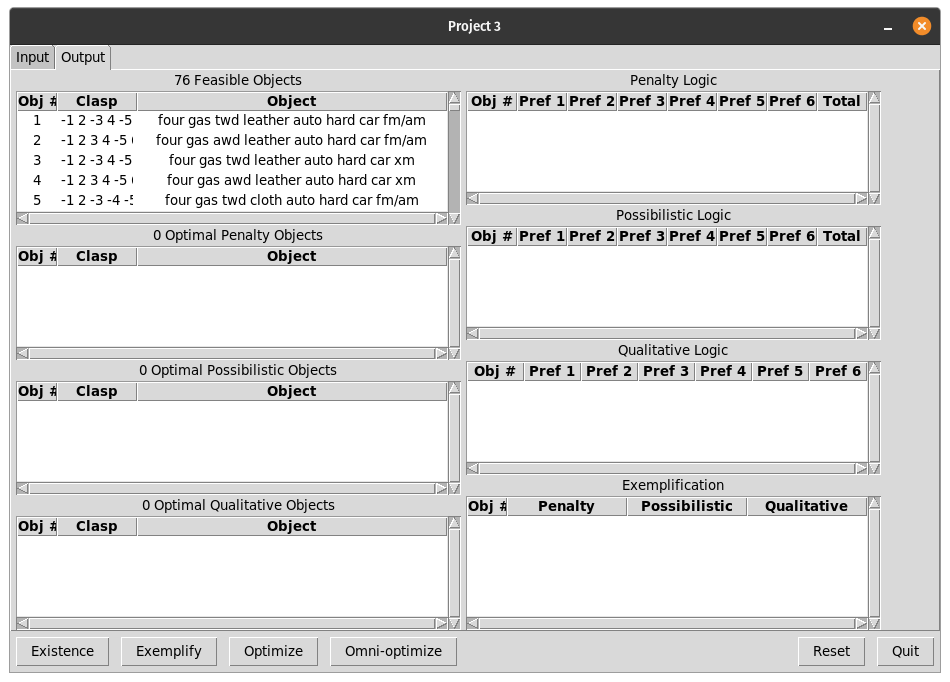
\includegraphics[scale=0.275,trim=1cm 1cm 1cm 1cm]{post_existence}
\caption{Screenshot of feasible objects output in table}
\end{center}
\end{figure}
\vspace{-2.5em}
\end{description}

\textbf{Note:} \\
Repetitive clicks of the existence button will always generate the same output in the table.

\section{Exemplification}
\vspace{.75em}
The following steps demonstrate the exemplification functionality of the program. \\
Comparing two random feasible objects based on each of the three preference logics.\\

\begin{description}[leftmargin=4em]
\item [Step 1:] Click the \textbf{"Exemplify"} button
\begin{figure}[H]
\begin{center}
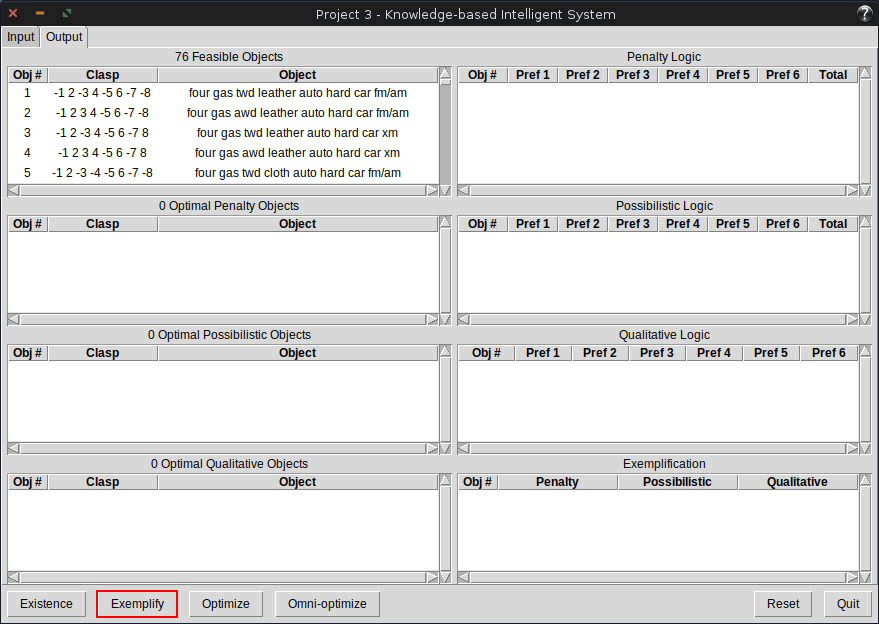
\includegraphics[scale=0.3,trim=1cm 1cm 1cm 1cm]{exemplify}
\caption{Screenshot of clicking the exemplify button}
\end{center}
\end{figure}
\vspace{-2.5em}
\item [Result:] The Penalty Logic, Possiblistic Logic, and Qualitative Choice Logic tables will be populated with the necessary underlying data used for exemplification. The \textbf{exemplification table} shows which objects are preferred for based on each logic.
\begin{figure}[H]
\begin{center}
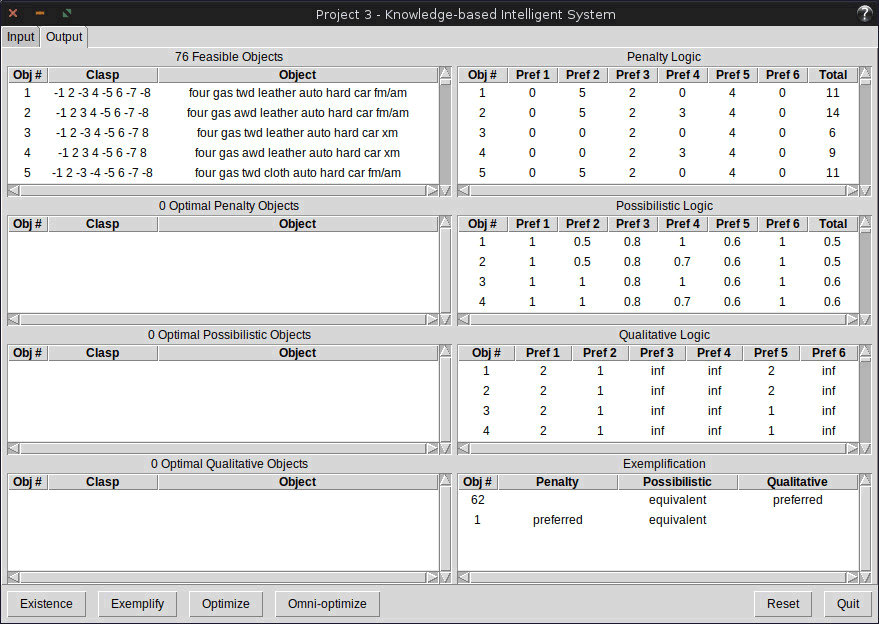
\includegraphics[scale=0.3,trim=1cm 1cm 1cm 1cm]{post_exemplify}
\caption{Screenshot of exemplification output in table}
\end{center}
\end{figure}
\vspace{-2.5em}
\end{description}
\textbf{Note:} \\
Repetitive clicks of the exemplify button will compare two different random feasible objects and generate different output in the table.

\section{Optimization}
The following steps demonstrate the optimization functionality of the program. \\
Showing a optimal feasible object based on each of the three preference logics.\\

\begin{description}[leftmargin=4em]
\item [Step 1:]  Click the \textbf{"Optimize"} button
\begin{figure}[H]
\begin{center}
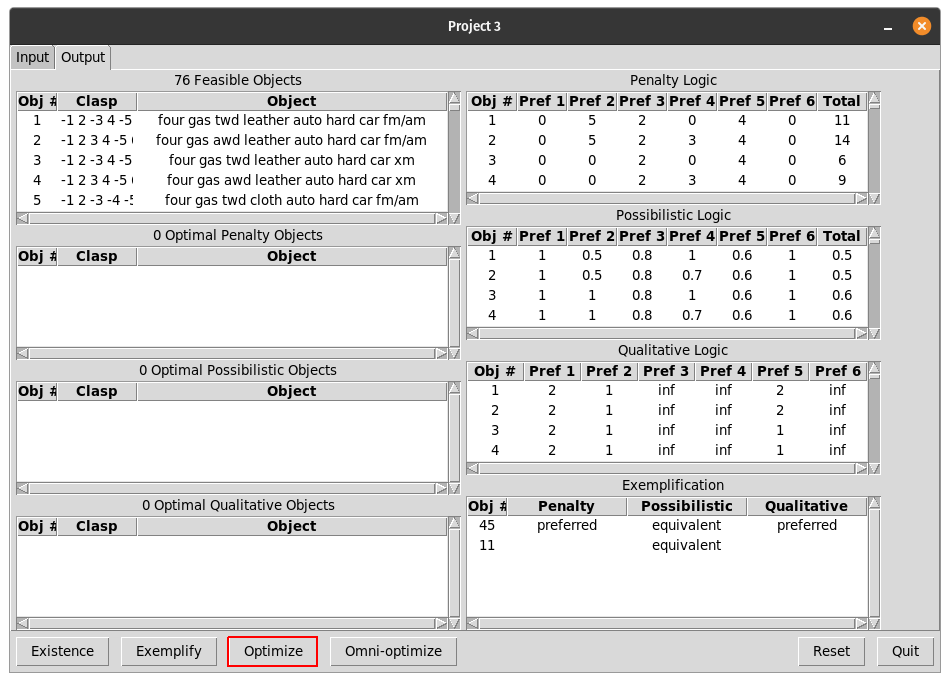
\includegraphics[scale=0.3,trim=1cm 1cm 1cm 1cm]{optimize}
\caption{Screenshot of clicking the optimize button}
\end{center}
\end{figure}
\vspace{-2.5em}
\item [Result:] The \textbf{Optimal Penalty Objects, Optimal Possiblistic Objects, and Optimal Qualitative Objects tables} will be populated with a single optimal object based on each logic.
\begin{figure}[H]
\begin{center}
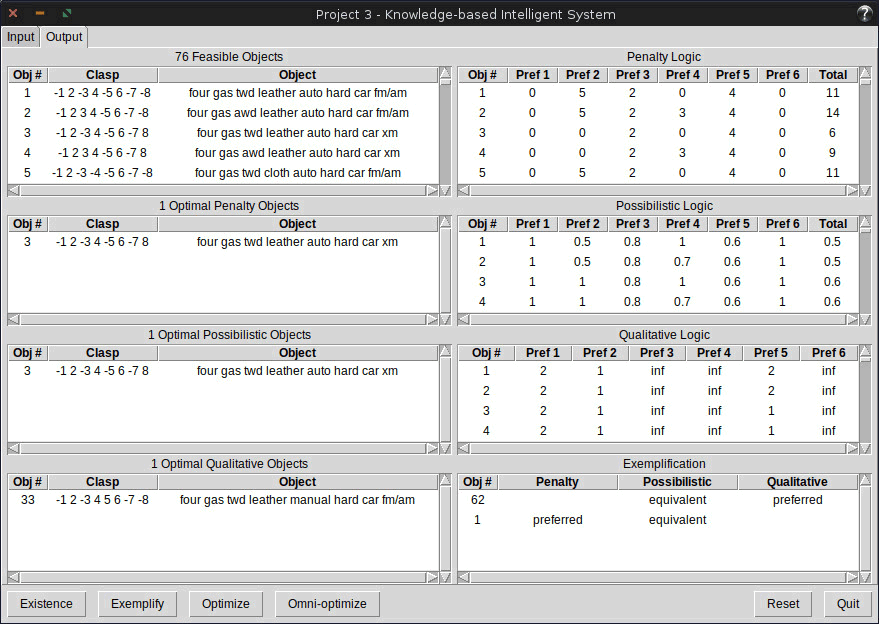
\includegraphics[scale=0.3,trim=1cm 1cm 1cm 1cm]{post_optimize}
\caption{Screenshot of optimization output in tables}
\end{center}
\end{figure}
\vspace{-2.5em}
\end{description}

\textbf{Note:} \\
Repetitive clicks of the optimize button will always generate the same output in the tables.

\section{Omni-Optimization}
The following steps demonstrate the omni-optimization functionality of the program. \\
Showing all optimal feasible objects based on each of the three preference logics.\\

\begin{description}[leftmargin=4em]
\item [Step 1:]  Click the \textbf{"Omni-Optimize"} button
\begin{figure}[H]
\begin{center}
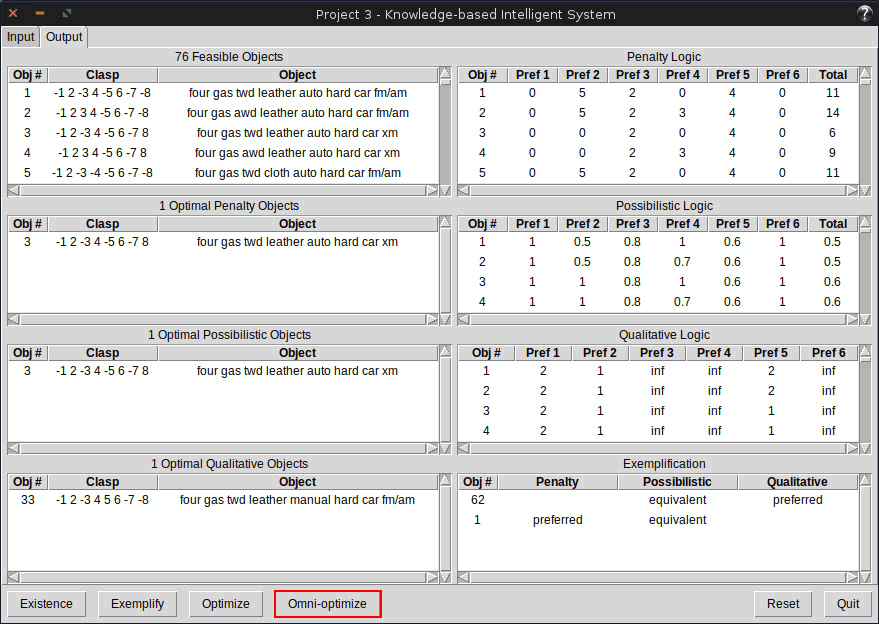
\includegraphics[scale=0.3,trim=1cm 1cm 1cm 1cm]{omni-optimize}
\caption{Screenshot of clicking the omni-optimize button}
\end{center}
\end{figure}
\vspace{-2.5em}
\item [Result:] The \textbf{Optimal Penalty Objects, Optimal Possiblistic Objects, and Optimal Qualitative Objects tables} will be populated with optimal objects based on each logic, along with the total number of optimal objects for each preference.
\begin{figure}[H]
\begin{center}
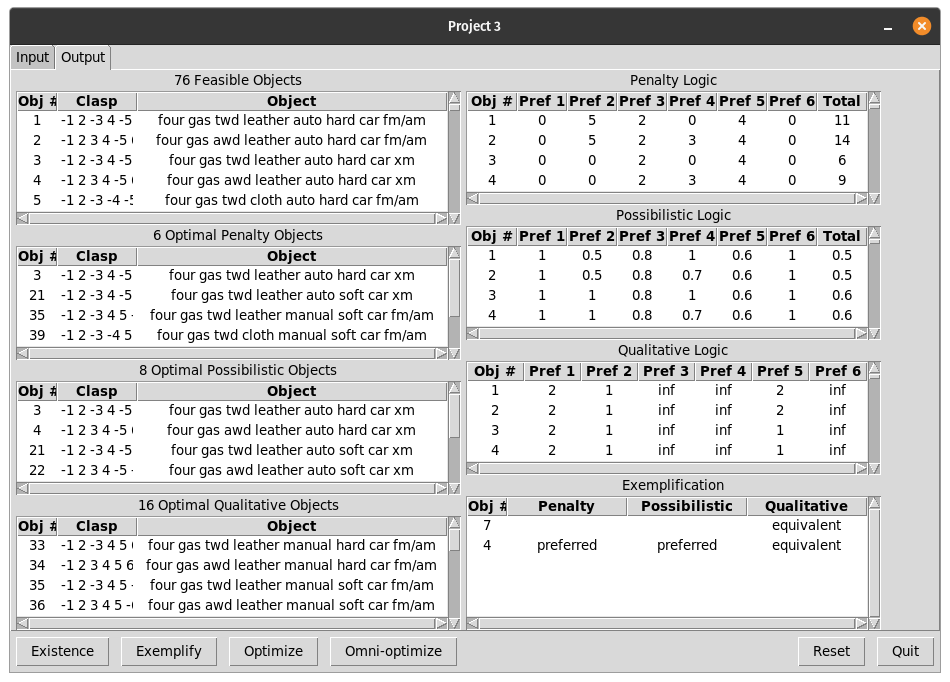
\includegraphics[scale=0.3,trim=1cm 1cm 1cm 1cm]{post_omni-optimize}
\caption{Screenshot of omni-optimization output in tables}
\end{center}
\end{figure}
\vspace{-2.5em}
\end{description}

\textbf{Note:} \\
Repetitive clicks of the omni-optimize button will always generate the same output in the tables.


\end{document}